\documentclass[10pt]{amsart}

\usepackage{algorithm}
\usepackage[noend]{algpseudocode}
\usepackage{amsfonts}
\usepackage{amsmath}
\usepackage{amssymb}
\usepackage{amsthm}
\usepackage[backend=biber, citestyle=numeric-comp, bibstyle=ieee]{biblatex}
\usepackage{changepage}
\usepackage{enumitem}
\usepackage{fancyhdr}
\usepackage{fontspec}
\usepackage{fullpage}
\usepackage[hidelinks]{hyperref}
\usepackage{mathtools}
\usepackage{physics}
\usepackage{tabularx}
\usepackage{thmtools}
\usepackage{tikz}
\usepackage{tikz-3dplot}
\usetikzlibrary{angles, cd, quantikz, quotes, patterns}
\usepackage{titlesec}
\usepackage{wasysym}

\usepackage{tikz-cd}

\usepackage{bookmark}
\usepackage[nameinlink]{cleveref}

\titleformat{\section}[runin]{\normalsize\bfseries}{\thesection}{1em}{}[]
\titleformat{\subsection}[runin]{\normalsize\bfseries}{\thesubsection}{1em}{}[]
\titleformat{\subsubsection}[runin]{\normalsize\bfseries}{\thesubsubsection}{1em}{}[]

\addbibresource{quantum_algorithms_for_lattice_problems_paper_notes.bib}

\theoremstyle{definition}
\newtheorem{theorem}{Theorem}
\newtheorem{definition}{Definition}
\theoremstyle{remark}
\newtheorem{problem}[theorem]{Problem}
\newtheorem{lemma}[theorem]{Lemma}
\newtheorem{remark}[theorem]{Remark}
\newtheorem{observation}[theorem]{Observation}
\newtheorem{example}[theorem]{Example}
\newtheorem{corollary}[theorem]{Corollary}

\renewcommand{\qedsymbol}{\(\blacksquare\)}

\setlength{\parindent}{0pt}

\DeclareMathOperator{\controrot}{CR}
\DeclareMathOperator{\expectation}{E}
\DeclareMathOperator{\gf}{GF}
\DeclareMathOperator{\qft}{QFT}
\DeclareMathOperator{\rk}{rk}
\DeclareMathOperator{\defect}{def}
\DeclareMathOperator{\swapgate}{SWAP}
\DeclareMathOperator{\che}{CHE}
\DeclareMathOperator{\poly}{poly}
\DeclareMathOperator{\Span}{Span}
\DeclareMathOperator{\diag}{diag}

\newcommand{\djk}{\delta_{j, k}}
\newcommand{\tlk}{\tilde{\lambda_k}}

\newcommand{\evalat}[2]{\left.{#1}\middle|\right._{#2}}

% SOURCE: https://tex.stackexchange.com/questions/296151/double-head-and-hook-arrow
\newcommand{\hookdoubleheadrightarrow}{%
    \hookrightarrow\mathrel{\mspace{-15mu}}\rightarrow
}

\newcommand{\draftcomment}[2]{\textcolor{#1}{#2}}

\newcommand{\measurementsymbol}{
    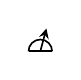
\begin{tikzpicture}[>=stealth, semithick, scale=1.5]
        \draw (-0.1, 0) -- (0.1, 0);
        \draw (0.1, 0) arc (0:180:0.1);
        \draw[->] (0, 0) -- (75:0.2);
    \end{tikzpicture}
}

\newcolumntype{L}[1]{>{\raggedright\arraybackslash}p{#1}}

\begin{document}
    valentinpi \hfill Last Change: July 23, 2024

    \section*{Notes on the Paper "Quantum Algorithms for Lattice Problems"} 

    \phantom{}

    In these notes, we will introduce some of the main concepts and a short summary of the recent preprint for a quantum algorithm for solving hard lattice problems by Yilei Chen \cite{Chen2024}.

    \section{Complex Gaussians and Karst Waves}

    The following is taken from \cite[pp. 3-4]{Chen2024}. Recall the Gaussian distribution \(\mathcal{N}(\mu, \sigma)\) for a continuous random variable given by the probability density function
    \begin{align}
        f(x) = \frac{1}{\sqrt{2\pi\sigma^2}} e^{-\frac{(x-\mu)^2}{2\sigma^2}}
    \end{align}
    with \(\mu \in \mathbb{R}\) being the mean and \(\sigma \in (0, \infty)\) being the standard deviation. The paper makes heavy use of so-called \emph{complex Gaussian states}. We define for some \(p \in \mathbb{R}_{\geq 1}\), \(P \coloneqq 2^p\), qubits and \(r \in \mathbb{R}_{> 0}\), acting as the deviation, the \emph{quantum Gaussian state}
    \begin{align}
        \ket{G_P^r} \coloneqq \sum_{x=0}^{P-1} \exp\left(-\pi\frac{x^2}{r^2}\right) \ket{x}
    \end{align}
    under omission of the appropriate normalization factor.

    \begin{figure}[!hbtp]
        \centering
        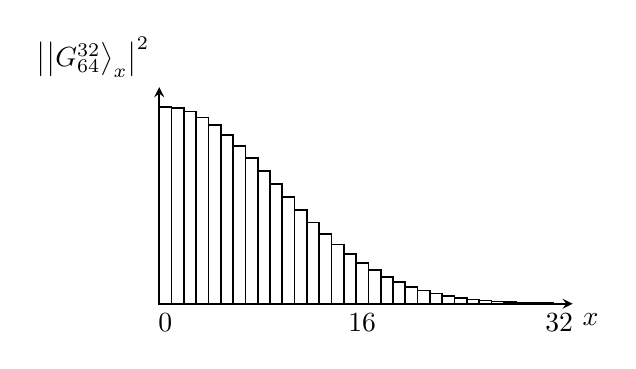
\begin{tikzpicture}[>=stealth, scale=2.5, semithick]
            \foreach \p in {0, ..., 32} {
                \pgfmathsetmacro{\y}{exp(-2*pi*\p^2/32^2)};
                \draw (\p/16, 0) rectangle ($(\p/16+1/16, \y)$);
            };
            \draw[->] (0, 0) -- (2.1, 0) node[below right] {\(x\)};
            \draw[->] (0, 0) -- (0, 1.1) node[above left] {\(\left|\ket{G_{64}^{32}}_x\right|^2\)};
            \node[below] at (0+1/32, 0) {\(0\)};
            \node[below] at (1+1/32, 0) {\(16\)};
            \node[below] at (2+1/32, 0) {\(32\)};
        \end{tikzpicture}
        \caption{Example squared amplitude distribution of a quantum Gaussian state.}
        \label{example_real_gaussian_state}
    \end{figure}
    
    Let \(s \in \mathbb{R}_{> 0}\) be the standard deviation for an imaginary part of a random variable. Append a number \(q \in \mathbb{N}_{\geq 1}\) of auxiliary qubits, \(Q \coloneqq 2^n\). Define the unitary \(U \in \mathbb{C}^{P \times P}\) with the action \(\ket{0} \mapsto \ket{G_P^r}\), which can be implemented using the technique of initializing a quantum state using an efficiently integrable probability distribution by Grover and Rudolph \cite{Grover}. We further define unitaries
    \begin{align}
        &U_0\colon \mathbb{C}^{PQ} \to \mathbb{C}^{PQ}, \ket{x}\ket{y} \mapsto \ket{x}\ket{y \oplus \mathcal{F}\left(\frac{x^2}{s^2}\right)} \text{ and }\\
        &U_1\colon \mathbb{C}^{Q} \to \mathbb{C}^{Q}, \ket{x} \mapsto e^{-\pi i x}\ket{x},
    \end{align}
    where \(\mathcal{F}(\cdot)\) denotes a bit representation of a floating real number. We compute
    \begin{align}
        \ket{0}^{\otimes (p+q)} &\xmapsto{U \otimes E_Q} \ket{G_P^r}\ket{0}^{\otimes q} \xmapsto{U_0} \sum_{x=0}^{P-1} \exp\left(-\pi\frac{x^2}{r^2}\right) \ket{x}\ket{\frac{x^2}{s^2}}\\
        &\xmapsto{U_0^\dagger(E_p \otimes U_1)} \sum_{x=0}^{P-1} \exp\left(-\pi\left(\frac{1}{r^2}+\frac{i}{s^2}\right)x^2\right) \ket{x}\ket{0}^{\otimes q},
    \end{align}
    also referred to as employing the \emph{Phase Kickback Trick}, all under omission of a normalization factor. implicitly defining the \emph{complex quantum Gaussian state} \(\ket{G_P^{r, s}}\). The parameters \(r\) and \(s\) control the spread of the real and imaginary parts of the amplitudes.

    \phantom{}

    Perform
    \begin{align}
        \ket{G_P^{r, s}} \xmapsto{\text{QFT}_P} \frac{1}{\sqrt{P}} \sum_{y=0}^{P-1}\sum_{x=0}^{P-1} \exp\left(-\pi\left(\frac{1}{r^2}+\frac{i}{s^2}\right)x^2\right)\exp\left(-2\pi i \frac{xy}{P}\right) \ket{y}.
    \end{align}
    It can be proven that the amplitudes of the resulting state concentrate on values of \(y\), which approximately lay on \(\alpha\mathbb{Z}\) for some \(\alpha \in \mathbb{R}_{> 0}\). The behavior of the real parts of the amplitudes is why they are referred to as \emph{Karst Waves}, see \Cref{karst_example}, resembling geological Karst formations, see \Cref{karst_inspiration}.
    \begin{figure}[!hbtp]
        \centering
        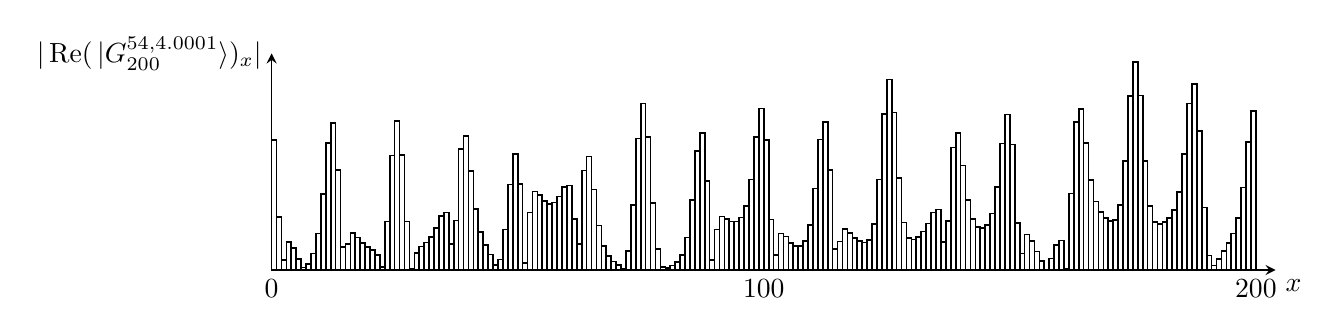
\begin{tikzpicture}[>=stealth, scale=2.5, semithick]
            %\foreach \p in {0, ..., 38} {
            %    \pgfmathsetmacro{\y}{exp(-pi*\p^2/32^2)*cos(-pi*\p^2/32^2-2*pi*\p*64/64)};
            %    \draw (\p/16, 0) rectangle ($(\p/16+1/16, \y)$);
            %};
            %\draw[->] (0, 0) -- (2.1, 0) node[below right] {\(x\)};
            %\draw[->] (0, 0) -- (0, 1.1) node[above left] {\(\Re(\ket*{G_{64}^{32, 32}}_x)\)};
            %\node[below] at (0+1/32, 0) {\(0\)};
            %\node[below] at (1+1/32, 0) {\(16\)};
            %\node[below] at (2+1/32, 0) {\(32\)};
            % >>> P, r, s = 200, 54, 4.0001
            % >>> [round(sum([exp(-pi*x**2/r**2) * cos(-pi/s**2*x**2-2*pi*x*y/P) for x in range(P)]), 4) for y in range(P)]
            \draw[->] (0, 0) -- (5.1, 0) node[below right] {\(x\)};
            \draw[->] (0, 0) -- (0, 1.1) node[left] {\(|\Re(\ket*{G_{200}^{54, 4.0001}})_x|\)};
            \node[below] at (0, 0) {0};
            \node[below] at (100*5/200, 0) {100};
            \node[below] at (200*5/200, 0) {200};
            \foreach \x/\y in {
                 0/ 5.2946,
                 1/ 2.1535,
                 2/ 0.3964,
                 3/ 1.1486,
                 4/ 0.8835,
                 5/ 0.4544,
                 6/ 0.0958,
                 7/ 0.2354,
                 8/ 0.6674,
                 9/ 1.4850,
                10/ 3.0832,
                11/ 5.1684,
                12/ 5.9699,
                13/ 4.0754,
                14/ 0.9370,
                15/ 1.0474,
                16/ 1.4999,
                17/ 1.3234,
                18/ 1.0991,
                19/ 0.9428,
                20/ 0.8205,
                21/ 0.6014,
                22/ 0.1236,
                23/ 1.9750,
                24/ 4.6471,
                25/ 6.0504,
                26/ 4.6769,
                27/ 1.9711,
                28/ 0.0646,
                29/ 0.6984,
                30/ 0.9503,
                31/ 1.1181,
                32/ 1.3472,
                33/ 1.7085,
                34/ 2.1889,
                35/ 2.3388,
                36/ 1.0667,
                37/ 2.0120,
                38/ 4.9301,
                39/ 5.4371,
                40/ 4.0164,
                41/ 2.4754,
                42/ 1.5381,
                43/ 1.0109,
                44/ 0.6257,
                45/ 0.2160,
                46/ 0.4264,
                47/ 1.6436,
                48/ 3.4778,
                49/ 4.7015,
                50/ 3.4939,
                51/ 0.2934,
                52/ 2.3338,
                53/ 3.1863,
                54/ 3.0532,
                55/ 2.8021,
                56/ 2.6949,
                57/ 2.7494,
                58/ 2.9840,
                59/ 3.3648,
                60/ 3.4312,
                61/ 2.0855,
                62/ 1.0613,
                63/ 4.0455,
                64/ 4.6200,
                65/ 3.2716,
                66/ 1.8120,
                67/ 0.9717,
                68/ 0.5674,
                69/ 0.3512,
                70/ 0.1976,
                71/ 0.0429,
                72/ 0.7850,
                73/ 2.6519,
                74/ 5.3398,
                75/ 6.7606,
                76/ 5.4075,
                77/ 2.7262,
                78/ 0.8498,
                79/ 0.1247,
                80/ 0.0784,
                81/ 0.1811,
                82/ 0.3246,
                83/ 0.6174,
                84/ 1.3255,
                85/ 2.8331,
                86/ 4.8401,
                87/ 5.5712,
                88/ 3.6104,
                89/ 0.4067,
                90/ 1.6456,
                91/ 2.1728,
                92/ 2.0841,
                93/ 1.9713,
                94/ 1.9732,
                95/ 2.1316,
                96/ 2.5961,
                97/ 3.6813,
                98/ 5.4151,
                99/ 6.5616,
               100/ 5.2946,
               101/ 2.0491,
               102/ 0.6103,
               103/ 1.4833,
               104/ 1.3586,
               105/ 1.1020,
               106/ 0.9715,
               107/ 0.9817,
               108/ 1.1899,
               109/ 1.8420,
               110/ 3.3130,
               111/ 5.2977,
               112/ 6.0181,
               113/ 4.0574,
               114/ 0.8642,
               115/ 1.1657,
               116/ 1.6562,
               117/ 1.5115,
               118/ 1.3142,
               119/ 1.1840,
               120/ 1.1224,
               121/ 1.2212,
               122/ 1.8689,
               123/ 3.6752,
               124/ 6.3292,
               125/ 7.7390,
               126/ 6.3968,
               127/ 3.7495,
               128/ 1.9337,
               129/ 1.3030,
               130/ 1.2416,
               131/ 1.3542,
               132/ 1.5596,
               133/ 1.8950,
               134/ 2.3442,
               135/ 2.4563,
               136/ 1.1390,
               137/ 1.9944,
               138/ 4.9786,
               139/ 5.5666,
               140/ 4.2464,
               141/ 2.8326,
               142/ 2.0607,
               143/ 1.7575,
               144/ 1.6977,
               145/ 1.8317,
               146/ 2.2907,
               147/ 3.3843,
               148/ 5.1386,
               149/ 6.3173,
               150/ 5.0952,
               151/ 1.9092,
               152/ 0.6729,
               153/ 1.4456,
               154/ 1.1889,
               155/ 0.7544,
               156/ 0.3725,
               157/ 0.0030,
               158/ 0.4614,
               159/ 1.0075,
               160/ 1.2011,
               161/ 0.0439,
               162/ 3.1098,
               163/ 6.0279,
               164/ 6.5478,
               165/ 5.1540,
               166/ 3.6568,
               167/ 2.7852,
               168/ 2.3554,
               169/ 2.1222,
               170/ 1.9944,
               171/ 2.0442,
               172/ 2.6540,
               173/ 4.4302,
               174/ 7.0597,
               175/ 8.4492,
               176/ 7.0895,
               177/ 4.4264,
               178/ 2.5950,
               179/ 1.9473,
               180/ 1.8646,
               181/ 1.9470,
               182/ 2.1099,
               183/ 2.4293,
               184/ 3.1692,
               185/ 4.7148,
               186/ 6.7674,
               187/ 7.5531,
               188/ 5.6586,
               189/ 2.5359,
               190/ 0.5843,
               191/ 0.1843,
               192/ 0.4385,
               193/ 0.7752,
               194/ 1.0988,
               195/ 1.4841,
               196/ 2.1210,
               197/ 3.3466,
               198/ 5.2012,
               199/ 6.4572
            }{
                \draw (\x*5/200, 0) rectangle (\x*5/200+5/200, \y/8);
            };
        \end{tikzpicture}
        \caption{Absolute values of the real parts of the amplitudes of \(\ket*{G_{200}^{54, 4.0001}}\), parameters taken from \cite[p. 5]{Chen2024}.}
        \label{karst_example}
    \end{figure}
    \begin{figure}[!hbtp]
        \centering
        \includegraphics[width=0.75\linewidth]{img/87340-Li-River_(29881879337).jpg}
        \caption{Example of Karst formations in Guilin, China, see \cite{Karst_China}.}
        \label{karst_inspiration}
    \end{figure}
    
    \section{Windowing with States} The following is due to \cite[pp. 4-6]{Chen2024}. \emph{Windowing} is a technique of combining two quantum states in a \emph{convolution}-type manner. The technique works as follows: Suppose two states
    \begin{align}
        \ket{\Phi} \coloneqq \sum_{x=0}^{P-1} \Phi_x \ket{x} \text{ and } \ket{\Psi} \coloneqq \sum_{y=0}^{Q-1} \Psi_y \ket{y}
    \end{align}
    are given. We tensorize both states and perform
    \begin{align}
        \ket{\Phi} \otimes \ket{\Psi} \xmapsto{U_{\text{Id}}} \sum_{x=0}^{P-1}\sum_{y=0}^{Q-1} \Phi_x\Psi_y \ket{x}\ket{x+y \bmod P} \xmapsto{E_P \otimes \measurementsymbol} \sum_{x=0}^{P-1} \Phi_x\Psi_{y' - x \bmod Q} \ket{x}\ket{y'}
    \end{align}
    with some \(y' = x+y \bmod Q\), the state obtained is the result.

    \section{Algorithm Outline}

    Recall the LWE (Learning With Errors) problem. On a high level, the task is to find a secret vector, whose entries are sampled from a distribution. Solving LWE in polynomial time gives polynomial algorithms for the SVP (Shortest Vector Problem) and its variants \cite[pp. 1-2]{Chen2024}.

    \begin{enumerate}[label=\arabic*., wide]
        \item In the algorithms preparatory phase, a given LWE instance is converted into a version with some chosen error terms following a secret distribution and then into a so-called \emph{\(q\)-ary lattice with a unique shortest vector} \cite[14-18]{Chen2024}, where \(q \in \mathbb{N}\). These reductions give a problem that is as hard to solve as normal LWE. Thus, the reduction roughly follows the strategy \(\text{SVP} \leq \text{LWE} \leq \text{SVP}\). The "\(q\)-ary" part of the lattice name implies the use of \(\mathbb{Z}_q\) to make the lattice finite for the algorithm, as a quantum register will be used to store a complex Gaussian superposition over the lattice.
        \item The preparation for the algorithm ends with a comprehensive parameter selection \cite[pp. 18-20]{Chen2024}.
        \item The main quantum algorithm consists of nine steps. In the first seven steps, an imaginary Gaussian state based on a superposition of the \(q\)-ary lattice is windowed with a special auxiliary state and processed further \cite[pp. 20-31]{Chen2024}.
        \item The result is then reduced to a linear system of equations over a finite field, which is supposed to yield the LWE solution \cite[pp. 31-39]{Chen2024}.
    \end{enumerate}

    \begin{table}[!hbtp]
        \centering
        \caption{Extended Paper Overview}
        \begin{tabular}{|c|L{10cm}|}
            \hline
             PDF Page & Description\\\hline
             1-2  & Abstract, Comment and Contents\\
             3-5  & Definitions of SVP, GapSVP, SIVP and LWE\\
             5-8  & Complex Gaussians\\
             8-10 & Reduced algorithm overview, very sparse on inner workings.\\
            10-11 & Preliminaries: Math\\
            12-14 & Preliminaries: Lattices\\
            14-16 & Preliminaries: Quantum Computation\\
            16-22 & Transform LWE in three steps: First with \(k\) known secrets by essentially adding \(k\) entries to the search vector, then into a \(q\)-ary SVP and then select parameters appropriately.\\
            22-24 & Detailed Quantum Algorithm Description\\
            24-40 & Description of Steps\\
            39    & Bug\\
            41-65 & Detailed proofs, further discussions, acknowledgements and references\\
            \hline
        \end{tabular}
    \end{table}

    \phantom{}
    
    We will not go into further detail here, but we will give a short description of the technique involved in the claimed problem of the algorithms analysis discovered on April 18, 2024.
    
    \phantom{}
    
    For that, we consider another technique used, called \emph{domain extension} \cite[p. 14]{Chen2024}. Suppose we are given a \(P\)-periodic function \(f\colon \mathbb{Z} \to \mathbb{C}\) with \(f(\mathbb{Z}_P) \neq \{0\}\). Define
    \begin{align}
        \ket{\phi} \coloneqq \sum_{x=0}^{P-1} f(x) \ket{x},
    \end{align}
    again omitting a normalization factor. Let \(c \in \mathbb{N}_{\geq 1}\), \(C \coloneqq 2^c\). We perform
    \begin{align}
        \ket{0}^{\otimes c}\ket{\phi} &\xmapsto{H^{\otimes c} \otimes E_P} \frac{1}{\sqrt{C}} \sum_{h=0}^{C-1}\sum_{x=0}^{P-1} f(x) \ket{h}\ket{x}\\
        &= \frac{1}{\sqrt{C}} \sum_{h=0}^{C-1}\sum_{x=0}^{P-1} f(hP+x) \ket{hP+x} = \frac{1}{\sqrt{C}} \sum_{x = 0}^{CP-1} f(x)\ket{x},
    \end{align}
    naturally extending the state from a superposition over \(\mathbb{Z}_P\) with amplitudes based on \(f\) to an analogous state over \(\mathbb{Z}_{CP}\).
    
    \phantom{}

    The algorithms analysis is claimed to fail due to a wrong application of the domain extension technique in step 9 \cite[pp. 34-38]{Chen2024}.

    \section{Further Perspectives}

    We have discussed four techniques used in the paper by Yilei: 
    \begin{itemize}
        \item Real and complex Gaussian states
        \item Karst wave states
        \item Windowing states
        \item Domain extension
    \end{itemize}
    Based on them, we will now discuss some possible directions and some more aspects to the algorithm.

    \phantom{}

    Let \(t \in \mathbb{N}_{\geq 1}\), \(T \coloneqq 2^t\). In the original HHL algorithm, an auxiliary state
    \begin{align}
        \sqrt{\frac{2}{T}}\sum_{\tau=0}^{T-1} \sin\left(\frac{\pi(\tau+\frac{1}{2})}{T}\right)\ket{\tau}
    \end{align}
    was initialized at the beginning of the algorithm \cite[p. 2]{Harrow}. It helps with obtaining good approximations of the given Hamiltonians energies/eigenvalues. Comparing \Cref{sketch_of_the_amplitudes}, a sketch of the amplitudes of an example of this state, and \Cref{example_real_gaussian_state}, we recognize the similarity, the former should imitate a general real Gaussian state. I proposed this interpretation between 2021-2022.
    
    \begin{figure}[!hbtp]
        \centering
        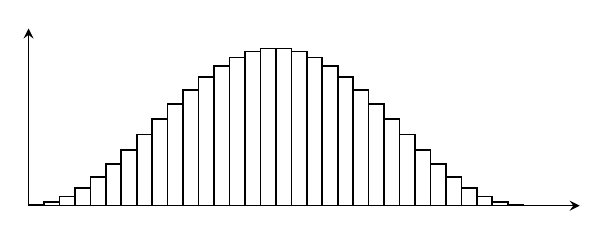
\begin{tikzpicture}[>=stealth, scale=2, semithick]
            \draw[->] (0, 0) -- (0, 1.125);
            \draw[->] (0, 0) -- (3.5, 0);
            \foreach \t in {0, 1, ..., 31} {
                \draw (pi * \t / 32, 0) rectangle ({pi * (\t + 1) / 32}, {16 * 2 / 32 * sin(180 / pi * pi * (\t + 0.5) / 32)^2});
            };
        \end{tikzpicture}
        \caption{Sketch of the amplitudes taken from \cite[p. 31]{valentinpi}, here for \(t = 5\) and scaled by \(16\).}
        \label{sketch_of_the_amplitudes}
    \end{figure}

    One might now ask the question if the original HHL algorithm is faster with a specifically chosen real or imaginary Gaussian quantum state.

    \phantom{}

    In terms of adiabatic quantum computation, one could study rapidly changing, Karst wave like, energy changes following the pattern of \Cref{karst_example}. There are no results on this yet, besides the trivial action of speeding up the adiabatic schedule employed. Fast changes of certain submatrices of a Hamiltonian might lead to an effect similar to the Zeno effect, effectively yielding an adiabatic version of the independent development of parts of a state, presenting a, possibly easier to control, alternative to the measurement-based Zeno.

    \phantom{}

    Windowing states may be useful for quantum machine learning - as it presents a natural version of convolution, as discussed above - or for techniques involving the modelling of an exponential number of signal samples using a quantum state, i.e., performing classical signal processing using a quantum state. There may exist results on this already. By the concept, and as complex Gaussian states, which are very important in general signal processing, have already been employed, it only seems natural to use the technique for this kind of signal processing.

    \phantom{}
    
    Domain extension does not seem to be an interesting technique in general, as it boils down to extending the domain of a periodic function, while it naturally keeps its image.

    \phantom{}

    As for the paper itself, work seems to have stopped fully, as indicated by Yileis note on the front page \cite{Chen2024}. Whilst the multiple techniques employed and the complexity of the arguments involved are intruiging, the paper fails to communicate the intuition and inner workings behind the proposed algorithm. Also, the fact that one application of domain extensions leads to the algorithm failing seems very strange, considering that domain extension does not add much information to a state, as discussed above.

    \phantom{}
    
    For now, following Yilei, it does not seem that the proposed result is still achievable due the bug. One possible opportunity for getting more people to work on it may be rewriting parts of the paper into a more pedagogical version, more clearly establishing notation (maybe by a notation table) and focusing more on the intuition behind the algorithm instead of its associated large formulas.

    \printbibliography{}
\end{document}
